\section{Fingertip detection}
In order to draw points using finger information, we have to detect the location of the fingertip.
If the posture is the ' pointing finger', we detect the fingertip of the index finger. 
If the posture is the 'palm', we detect the fingertip of the middle finger. \par
We assume that the fingertip is the furthest point from the center of the mass that is on the opposite side of the wrist .
Our environment allows us to assume the wrist side is always top of the image, so we can simply find the furthest point from the center of the mass among the bottom half of the mask.

This function is implemented in fingertip.py. 

Fig. \ref{fig:finger} shows the results of the fingertip detection.
This method detects the finger tip correctly when the posture is one finger or two fingers.
When the posture is a palm, the method sometimes detects the location between the middle finger and the other fingers.
Table \ref{tb:finger} shows the result of the detected fingertip when the posture is 'palm'.
We tried 143 frames of this posture.
The error rate is 12 \%. Fig. \ref{fig:errorfinger} shows the examples of failure. As we can see, it fails when the hand is not on the canvas. This would cause an error of about 10 pixels in the input  image and 20 pixels on the output canvas, which is about 3\% of the average length of the canvas.

\begin{figure}[htbp]
 \centering
 \begin{tabular}{lllll}
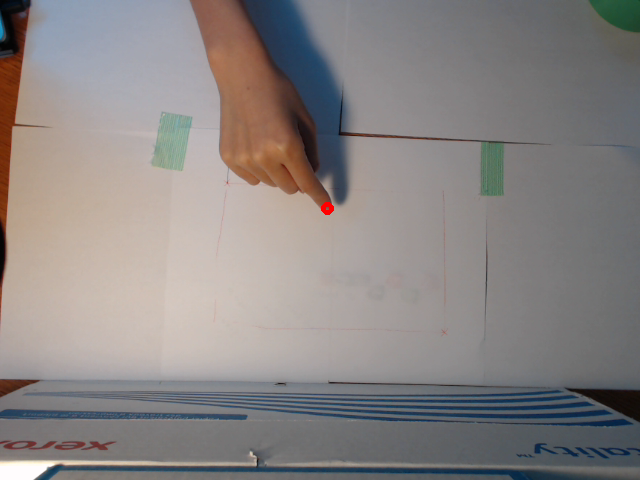
\includegraphics[width=5cm]{fig3/im1_13.png} &
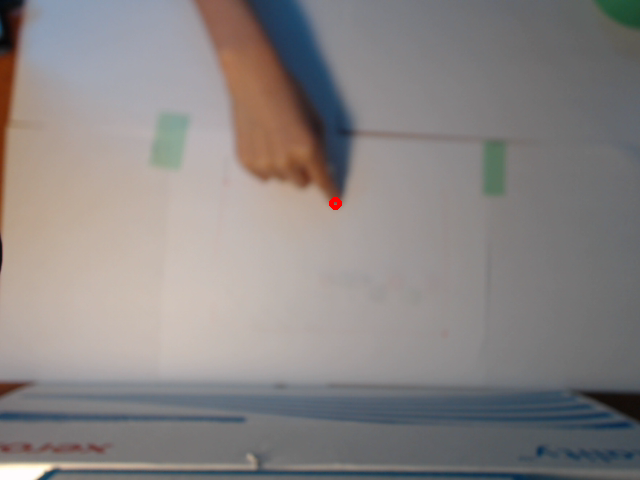
\includegraphics[width=5cm]{fig3/im1_55.png} \\
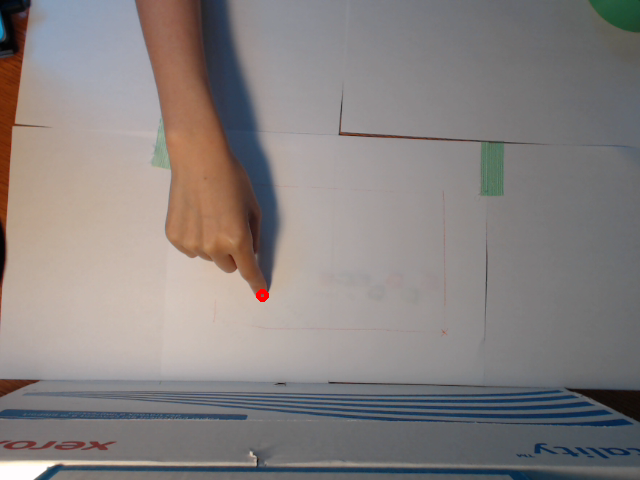
\includegraphics[width=5cm]{fig3/im1_67.png} &
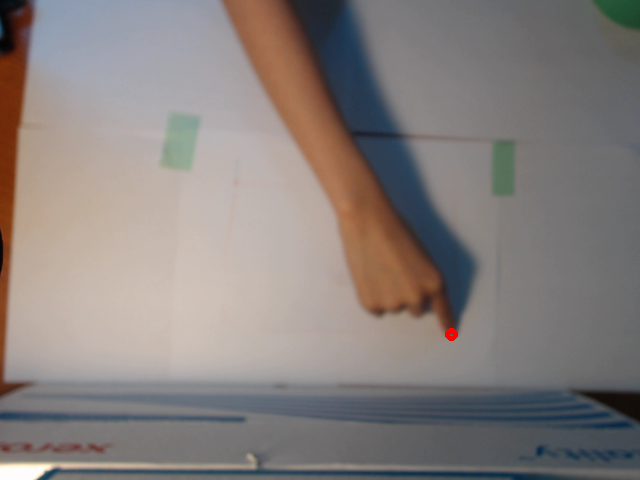
\includegraphics[width=5cm]{fig3/im1_146.png} \\
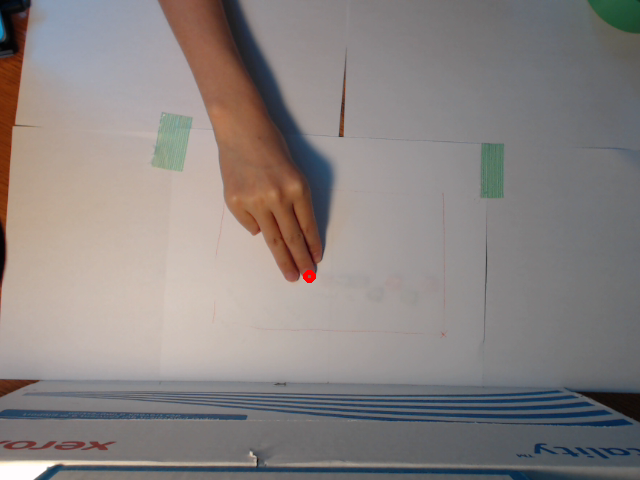
\includegraphics[width=5cm]{fig3/im2_26.png} &
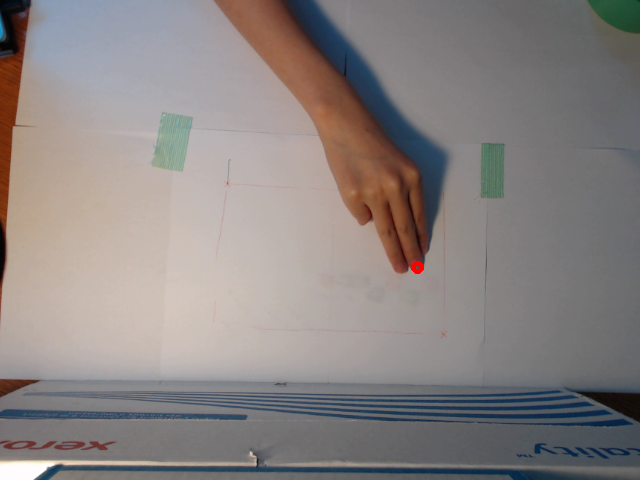
\includegraphics[width=5cm]{fig3/im2_98.png} \\
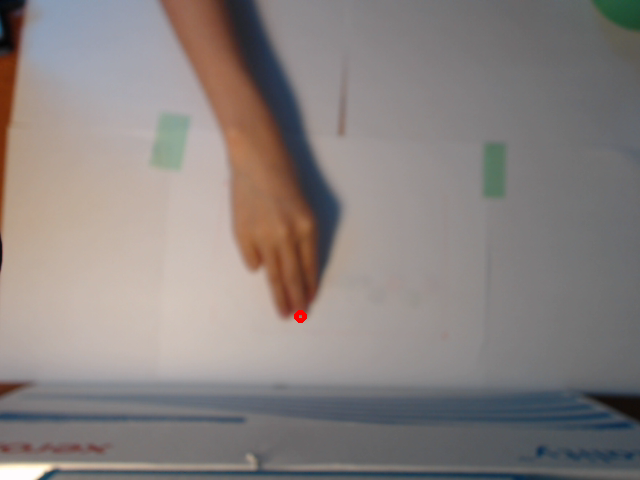
\includegraphics[width=5cm]{fig3/im2_149.png} &
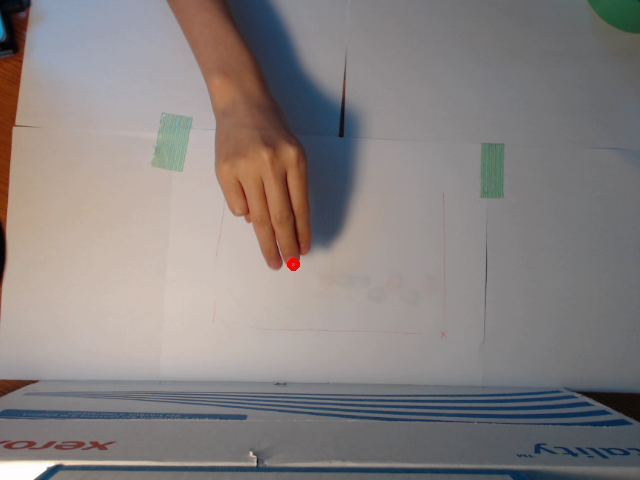
\includegraphics[width=5cm]{fig3/im2_162.png} \\
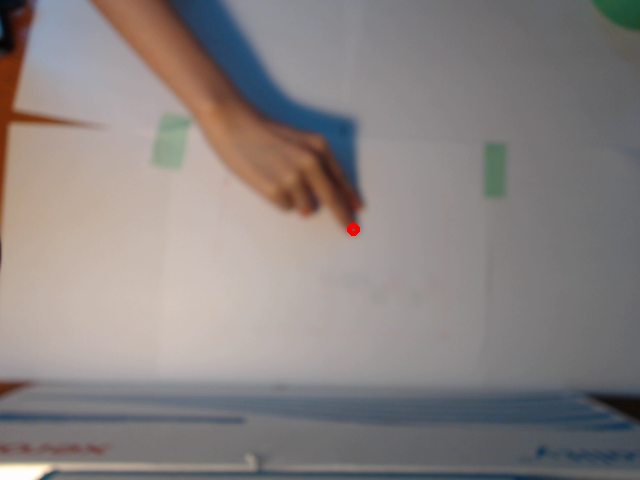
\includegraphics[width=5cm]{fig3/im3_78.png} &
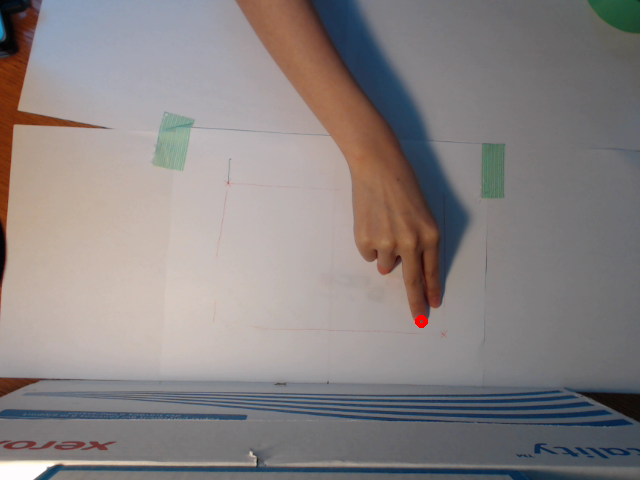
\includegraphics[width=5cm]{fig3/im3_109.png} \\
\end{tabular}

 \caption{The results of finger detection}
\label{fig:finger}
\end{figure}

\begin{figure}[htbp]
 \centering
 \begin{tabular}{lll}
	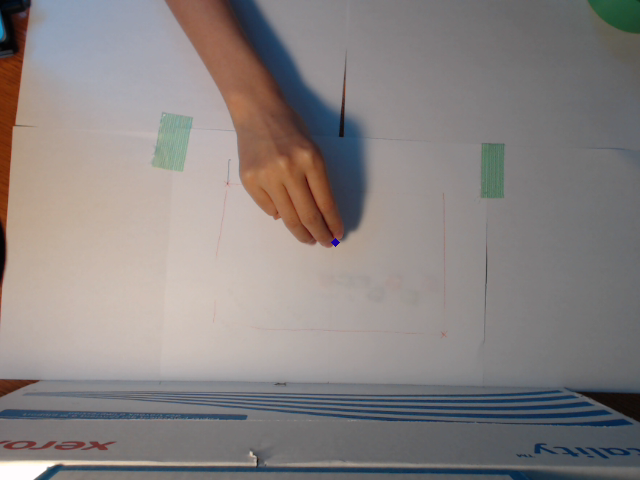
\includegraphics[width=5cm]{fig2/im2_109.png} &
	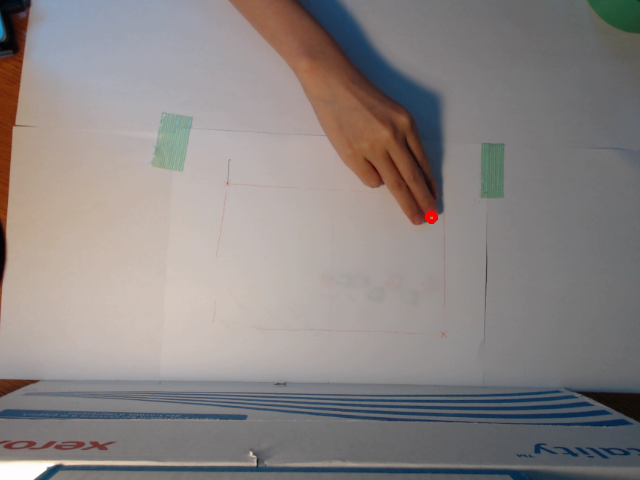
\includegraphics[width=5cm]{fig2/im2_133.png} \\
  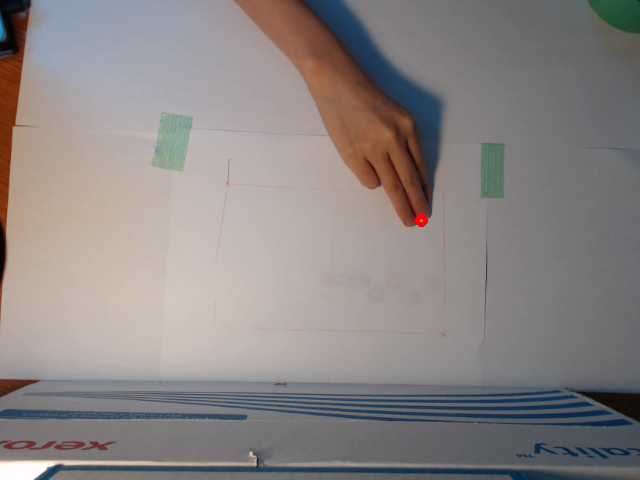
\includegraphics[width=5cm]{fig2/im2_138.png}&
	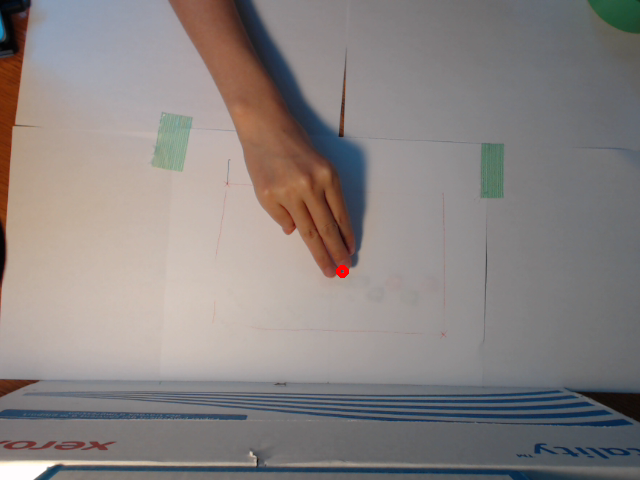
\includegraphics[width=5cm]{fig2/im2_4.png}  \\
	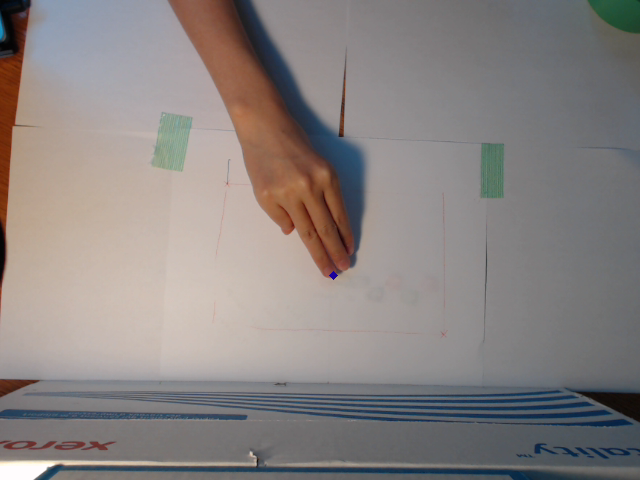
\includegraphics[width=5cm]{fig2/im2_5.png}  &
	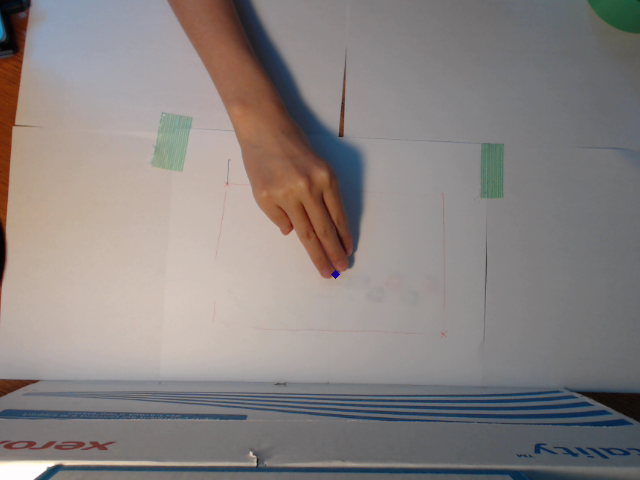
\includegraphics[width=5cm]{fig2/im2_6.png}
\end{tabular}

 \caption{The errors}
\label{fig:errorfinger}
\end{figure}

\begin{table}
 \caption{The result of three fingers' finger tip detection}
 \label{tb:finger}
 \begin{tabular}{|c|c|}
 \hline
 The location of the result &  \\ \hline
 Index finger & 0(0\%) \\ \hline
 Between index finger and middle finger & 1(0\%) \\ \hline
 Middle finger & 124 (87\%) \\ \hline
 Between middle finger and third finger & 12(8\%) \\ \hline
 Third finger & 6(4\%) \\ \hline
 Total & 143 \\ \hline
 \end{tabular}
\end{table}
